
\section{\trContactType\trHypersurface{}与温斯坦猜想}
\label{sec:contact-type-weinstein}

\hzsync{theorem}{5}
\hzsync{proposition}{4}
\hzsync{lemma}{2}

下面我们再挑出\trHypersurface{}的另一种\trSymplectic{}性质，它保证%
\trClosedCharacteristic{}的存在性。受 $\R^{2n}$ 中\trConvex{}与%
\trStarShaped{}\trEnergySurface{}的首批整体性结果的推动，A.~\trWeinstein{}在%
文献 [226] 中引入了下述概念：

\begin{definition}\label{def:contact-type}
\trSymplecticManifold{} $(M,\omega)$ 中一张\trCompact{}且\trOrientable{}的%
\trHypersurface{} $S\subset M$ 称为是\trContactType{}的，如果在 $S$ 上存在一个%
\trOneForm{} $\alpha$ 满足
\begin{align*}
\text{(i)}\qquad & d\alpha\ =\ j^{*}\omega\\
\text{(ii)}\qquad & \alpha(\xi)\ \neq\ 0\qquad\text{对}\quad0\neq\xi\in\mathcal{L}_{S}\ ,
\end{align*}
其中 $j:S\to M$ 是\trInclusionMapping，而 $\mathcal{L}_{S}$ 是 $S$ 的%
\trCharacteristicLineBundle。
\end{definition}

由于 $\xi\in\mathcal{L}_{S}$ 位于 $\omega|S$ 的\trKernel{}之中且%
$\alpha(\xi)\neq0$，故由 $\ker\alpha(x)=\bigl\{\eta\in T_{x}S\ \bigm|\ %
\alpha_{x}(\eta)=0\bigr\}$ 给出的 $\alpha$ 的\trKernel{}是 $T_{x}S$ 的一个%
$(2n-2)$ 维\trSubspace，2-形式 $\omega$ 在其上是\trNondegenerate{}的，从而%
$d\alpha$ 亦然。于是，$\alpha\wedge(d\alpha)^{n-1}$ 是 $S$ 上的一个%
\trVolumeForm。从几何上看，1-形式 $\alpha$ 在 $S$ 上定义了一个\trSmooth{}的%
\trHyperplane{}场，它是奇数维\trManifold{} $S$ 上\textbf{\trContactStructure}%
（contact structure）的一个例子。

\textbf{A.~\trWeinstein{}猜想（1978）：}\quad\trContactType{}的且满足%
$H^{1}(S)=0$ 的\trHypersurface{} $S$ 必带有一条\trClosedCharacteristic。

我们将验证这个猜想——但不借助拓扑假设 $H^{1}(S)=0$，而是在一个%
\trSymplectic{}的假设之下：$S$ 有一个\trCapacity{}有限的\trNeighborhood{}%
$U\subset M$，即 $c_{0}(U,\omega)<\infty$。我们首先依循 A.~\trWeinstein{}%
[226] 把\trContactType{}这一概念重新表述如下：

\begin{proposition}\label{prop:contact-type-equiv}
\trCompact\trHypersurface{} $S\subset M$ 是\trContactType{}的，当且仅当存在一个%
定义在 $S$ 的\trNeighborhood{} $U$ 上的\trVectorField{} $X$，满足
\begin{align*}
\text{(i)}\qquad & L_{X}\omega\ =\ \omega\qquad\text{在 $U$ 上}.\\
\text{(ii)}\qquad & X(x)\ \notin\ T_{x}S\qquad\text{若}\quad x\in S\ .
\end{align*}
亦即，$X$ 与 $S$ \trTransversal。
\end{proposition}

为了证明这个命题，我们从一个\trPoincare{}型引理入手。

\begin{lemma}\label{lem:poincare-type-lemma}
设 $\pi:E\to N$ 是一个\trVectorBundle，并设 $\alpha$ 是 $E$ 上一个\trClosed{}%
的 $k$-形式，满足 $j^{*}\alpha=0$，这里\trInclusionMapping{} $j:N\to E$ 是该%
\trBundle{}的\textbf{零\trSection}（zero section）。那么，存在 $E$ 上一个%
$(k-1)$-形式 $\beta$ 满足
\[
\alpha\ =\ d\beta\qquad\text{以及}\qquad\beta|N\ =\ 0\ .
\]
\end{lemma}
\begin{proof}
利用各\trFiber{}的\trLinear{}结构，我们可以对 $t>0$ 定义沿\trFiber{}方向经%
乘法而作的\textbf{\trContractionMap}（contraction maps）$\varphi^{t}:E\to E$：%
$\varphi^{t}(x)=t\cdot x$。我们用 $X_{t}$ 表示由这族\trDiffeomorphism{}所%
生成的 $E$ 上的\trTimeDependent\trVectorField，按通常方式由%
$\frac{d}{dt}\varphi^{t}(x)=X_{t}\bigl(\varphi^{t}(x)\bigr)$（$t>0$）给出。%
若定义 $X_{1}(x)=\frac{d}{dt}\varphi^{t}(x)\big|_{t=1}\in T_{x}E$，我们便有%
表示 $X_{t}(x)=\frac{1}{t}X_{1}(x)$；此外，当 $x\in N$ 时 $X_{t}(x)=0$。%
利用 $d\alpha=0$，由\trCartan{}公式我们得到
\[
\frac{d}{dt}\bigl(\varphi^{t}\bigr)^{*}\alpha\ =\ \bigl(\varphi^{t}\bigr)^{*}%
L_{X_{t}}\alpha\ =\ d\Bigl\{\bigl(\varphi^{t}\bigr)^{*}i_{X_{t}}\alpha\Bigr\},
\]
其中
\[
\bigl(\varphi^{t}\bigr)^{*}i_{X_{t}}\alpha(x)\ =\ \alpha(t\cdot x)%
\Bigl(\frac{1}{t}\,d\varphi^{t}X_{1}(x),\ d\varphi^{t}\cdot\Bigr).
\]
由于 $\lim_{t\to0}\bigl(\varphi^{t}\bigr)^{*}\alpha=\pi^{*}j^{*}\alpha=0$ 且%
$\varphi^{1}(x)=x$，我们得出
\begin{align*}
\alpha\ &=\ \bigl(\varphi^{1}\bigr)^{*}\alpha-\lim_{t\to0}\bigl(\varphi^{t}\bigr)^{*}\alpha\\
&=\ \lim_{t\to0}\int_{t}^{1}\frac{d}{d\sigma}\bigl(\varphi^{\sigma}\bigr)^{*}\alpha\,d\sigma\\
&=\ d\int_{0}^{1}\Bigl(\bigl(\varphi^{\sigma}\bigr)^{*}i_{X_{\sigma}}\alpha\Bigr)d\sigma\ =\ d\beta
\end{align*}
对 $E$ 上一个\trSmooth{}的 $(k-1)$-形式 $\beta$ 成立。若 $x\in N$，则%
$X_{t}(x)=0$，从而 $i_{X_{t}}\alpha=0$，于是 $\beta(x)=0$。引理证毕。
\end{proof}

我们将利用这个引理把 $S$ 上的 1-形式 $\alpha$ 延拓到 $S$ 的一个开%
\trNeighborhood{}上去。

\begin{lemma}\label{lem:extend-contact-form}
若 $S\subset(M,\omega)$ 是\trContactType{}的，则在 $S$ 的一个\trNeighborhood{}%
$U$ 上存在一个 1-形式 $\tau$ 满足
\begin{align*}
\text{(i)}\qquad & d\tau\ =\ \omega\qquad\text{在 $U$ 上}\\
\text{(ii)}\qquad & j^{*}\tau\ =\ \alpha\qquad\text{在 $S$ 上}
\end{align*}
其中 $j:S\to U$ 是\trInclusionMapping。
\end{lemma}
\begin{proof}
由于 $S$ 是\trCompact{}且\trOrientable{}的，故存在一个\trDiffeomorphism{}%
$\psi:S\times(-1,1)\to U$，它映到 $S$ 的一个开\trNeighborhood{} $U$ 上，并且%
对一切 $x\in S$ 满足 $\psi(x,0)=x$。这已在前一节中证明。于是，从%
$S\times(-1,1)$ 到 $S$ 上的\trProjection{}映射 $(x,t)\mapsto x$ 便诱导出一个%
\trSmooth{}映射 $r:U\to S$，它在 $S$ 上是\trIdentityMap。在 $U$ 上定义%
1-形式 $\mu=r^{*}\alpha$，则 $j^{*}\mu=j^{*}r^{*}\alpha=\alpha$。现在考察%
$U$ 上的 2-形式 $\omega-d\mu$。此时
\[
d(\omega-d\mu)\ =\ d\omega\ =\ 0,
\]
这是因为\trSymplecticStructure{}是一个\trClosed{}形式。此外，利用%
$j^{*}\omega=d\alpha$，
\[
j^{*}(\omega-d\mu)\ =\ d\alpha-d(j^{*}\mu)\ =\ d\alpha-d\alpha\ =\ 0\ .
\]
由于 $U$ \trDiffeomorphic{}于 $S\times(-1,1)$，而后者又\trIsomorphic{}于%
\trBundle{} $S\times\R$，我们可把\cref{lem:poincare-type-lemma}应用于 2-形式%
$\omega-d\mu$，从而找到一个 1-形式 $\vartheta$ 满足 $\omega-d\mu=d\vartheta$%
与 $j^{*}\vartheta=0$。于是，若在 $U$ 上定义 1-形式 $\tau=\mu+\vartheta$，%
我们便得到 $d\tau=d(\mu+\vartheta)=\omega$ 与 $j^{*}\tau=j^{*}\mu=\alpha$，%
正如引理所要求。
\end{proof}

现在我们已经为证明\cref{prop:contact-type-equiv}做好了准备。

\begin{proof}
设 $S\subset M$ 是\trContactType{}的。于是，取\cref{lem:extend-contact-form}的%
1-形式 $\tau$，我们可以在 $U$ 上用
\[
i_{X}\omega\ =\ \tau\qquad\text{在}\quad U\ .
\]
定义\trVectorField{} $X$。这个\trVectorField{}便具有该命题所要求的诸性质。%
的确，由\cref{lem:extend-contact-form}，%
$\omega=d\tau=d(i_{X}\omega)=-i_{X}(d\omega)+L_{X}\omega=L_{X}\omega$，%
剩下的只需证明 $X$ 与 $S$ \trTransversal。若 $0\neq\xi\in\mathcal{L}_{S}(x)$，%
则
\[
\omega\Bigl(X(x),\xi\Bigr)\ =\ \tau(\xi)\ =\ \alpha(\xi)\ \neq\ 0
\]
这来自对 $\alpha$ 的假设。由于按定义 $\xi$ 属于 $\omega$ 限制到%
\trTangentSpace{} $T_{x}S$ 上的\trKernel，我们得出 $X(x)\notin T_{x}S$。

反之，若\trVectorField{} $X$ 满足该命题的假设 (i) 与 (ii)，我们在 $U$ 上定义%
1-形式
\[
\alpha\ =\ i_{X}\omega\ .
\]
于是 $d\alpha=d(i_{X}\omega)=L_{X}\omega=\omega$，并且由\trTransversal{}条件%
$X(x)\notin T_{x}S$，对 $0\neq\xi\in\mathcal{L}_{S}(x)$ 我们得出%
$0\neq\omega\Bigl(X(x),\xi\Bigr)=\alpha(\xi)$。用这个 1-形式 $\alpha$，我们已%
验证了 $S$ 是\trContactType{}的。命题证毕。
\end{proof}

$S$ 为\trContactType{}这一性质的重要意义在于：$S$ 容许一个特定的以 $S$ 为%
模型的\trParameterizedHypersurfaceFamily{} $(S_{\varepsilon})$；它由%
\cref{prop:contact-type-equiv}所保证的那个特殊\trVectorField{} $X$ 的\trFlow{}%
$\varphi^{t}$ 来定义。由于 $S$ \trCompact{}且 $X$ 与 $S$ \trTransversal，%
映射
\[
\psi\ :\ S\times(-\varepsilon,\varepsilon)\ \to\ U\subset M
\]
——它由 $\psi(x,t)=\varphi^{t}(x)$（$x\in S$，$\lvert t\rvert<\varepsilon$）%
定义——在 $\varepsilon>0$ 充分小时是到 $S$ 的一个开\trNeighborhood{} $U$ 上的%
\trDiffeomorphism。由 $L_{X}\omega=\omega$ 我们得出%
$\frac{d}{dt}\bigl(\varphi^{t}\bigr)^{*}\omega=\bigl(\varphi^{t}\bigr)^{*}%
L_{X}\omega=\bigl(\varphi^{t}\bigr)^{*}\omega$。于是，由 $\varphi^{0}=id$，
\[
\bigl(\varphi^{t}\bigr)^{*}\omega\ =\ e^{t}\omega\ .
\]
现在设 $\xi\in\mathcal{L}_{S}(x)$，则对一切 $\eta\in T_{x}S$
\[
0\ =\ \omega(\xi,\eta)\ =\ e^{t}\omega(\xi,\eta)\ =\ \bigl(\varphi^{t}\bigr)^{*}%
\omega(\xi,\eta)\ =\ \omega\Bigl(d\varphi^{t}(x)\xi,\ d\varphi^{t}(x)\eta\Bigr),
\]
从而 $d\varphi^{t}(x)\xi\in\mathcal{L}_{S_{t}}\bigl(\varphi^{t}(x)\bigr)$。%
我们看到
\[
T\varphi^{t}\ :\ \mathcal{L}_{S}\ \to\ \mathcal{L}_{S_{t}}
\]
是\trVectorBundle{}之间的一个\trIsomorphism。于是，$\varphi^{t}$ 通过%
$P\mapsto\varphi^{t}(P)$ 在诸\trClosedCharacteristic{}之间诱导出一个一一对应
\[
\mathcal{P}(S)\ \longleftrightarrow\ \mathcal{P}(S_{t})
\]
这把我们引向下述定义：

\begin{definition}\label{def:stable-hypersurface}
\trCompact\trHypersurface{} $S\subset(M,\omega)$ 称为\trStable{}的，如果存在%
一个以 $S$ 为模型的\trParameterizedHypersurfaceFamily{} $(S_{\varepsilon})$，%
它具有下述附加性质：与之相配的\trDiffeomorphism{} $\psi:S\times(-1,1)\to U$%
诱导出\trBundle\trIsomorphism
\[
T\psi_{\varepsilon}\ :\ \mathcal{L}_{S}\ \to\ \mathcal{L}_{S_{\varepsilon}}\ ,
\]
对每个 $\varepsilon\in(-1,1)$ 成立。
\end{definition}

正如我们刚刚证明的，\trContactType{}的\trHypersurface{}是\trStable{}的。然而，%
\trStable{}的\trHypersurface{}未必是\trContactType{}的，下面的例子说明了这%
一点。考察\trSymplecticManifold{} $M=N\times\R^{2}$，其\trSymplecticStructure{}%
为 $\omega=\omega_{1}\oplus\omega_{0}$，其中 $(N,\omega_{1})$ 是一个无%
\trBoundary{}的\trCompact\trSymplecticManifold。考察\trHypersurface
\[
S\ =\ N\times\Bigl\{|z|^{2}=1\Bigr\}\ \subset\ M
\]
并把\trParametrization{} $\psi:S\times(-1,1)\to M$ 定义为%
$\psi\bigl((x,z),\varepsilon\bigr)=(x,(1+\varepsilon)z)$，于是%
$S_{\varepsilon}=N\times\bigl\{|z|^{2}=(1+\varepsilon)^{2}\bigr\}$\footnote{原书印作「$\psi((x,z),\varepsilon)=(x,\varepsilon z)$」与「$S_{\varepsilon}=N\times\{|z|^{2}=\varepsilon^{2}\}$」，如此则 $\varepsilon=0$ 时整张圆周塌缩为一点，既非微分同胚亦不满足 $S_{0}=S$，此处按文义径改。——译者注}。显然 $S$ 是%
\trStable{}的，但 $S$ 不是\trContactType{}的。否则，我们将在 $S$ 上找到一个%
满足 $d\alpha=j^{*}\omega$ 的 1-形式 $\alpha$，这里 $j:S\to M$ 是%
\trInclusionMapping。以 $i:N\to N\times\bigl\{(1,0)\bigr\}$ 记 $N$ 到 $S$ 中的%
\trInclusionMapping，我们推得
\[
i^{*}(d\alpha)\ =\ i^{*}j^{*}\omega\ =\ \omega_{1}\ .
\]
于是，\trSymplectic{}形式 $\omega_{1}=d(i^{*}\alpha)$ 必是\trExact{}的。然而%
这是不可能的。的确，由\trStokes{}定理
\[
\operatorname{vol}(N)\ =\ \int_{N}\omega_{1}\wedge\ldots\wedge\omega_{1}\ =\ 0,
\]
可知 $\omega_{1}^{(n)}$ 不是一个\trVolumeForm，从而 $\omega_{1}$ 是%
\trDegenerate{}的，这与 $\omega_{1}$ 是一个\trSymplectic{}形式的假设相矛盾。

按定义，一个\trStable{}的\trHypersurface{} $S$ 容许一个具有下述性质的%
\trParameterizedHypersurfaceFamily{} $(S_{\varepsilon})$：只要对单独一个%
$\varepsilon\in(-1,1)$ 有 $\mathcal{P}(S_{\varepsilon})\neq\emptyset$，便有%
$\mathcal{P}(S)\neq\emptyset$。于是，我们从\cref{thm:hz-dense-parameterized}%
推得下述整体存在性陈述：

\begin{theorem}\label{thm:stable-implies-closed}
设\trCompact\trHypersurface{} $S\subset(M,\omega)$ 容许一个\trCapacity{}有限%
的\trNeighborhood{} $U$：$c_{0}(U,\omega)<\infty$。若 $S$ 此外还是\trStable{}的，%
则
\[
\mathcal{P}(S)\ \neq\ \emptyset\ .
\]
\end{theorem}

特别地，若 $S$ 是\trContactType{}的，则 $\mathcal{P}(S)\neq\emptyset$\footnote{原书印作「$\mathcal{P}(S)\neq 0$」，疑为「$\neq\emptyset$」之误，此处径改。——译者注}。

$\bigl(\R^{2n},\omega_{0}\bigr)$ 中的\trCompact\trHypersurface{}总具有一个%
\trCapacity{} $c_{0}$ 有限的有界\trNeighborhood，于是我们从%
\cref{thm:stable-implies-closed}推得 C.~\trViterbo{} [217] 在 1987 年给出的、%
对 A.~\trWeinstein{}猜想的那个著名的解决。至于另一个证明，我们提及 [45]%
（1988）。

\begin{theorem}[C.~\trViterbo]\label{thm:viterbo-contact-type}
$\bigl(\R^{2n},\omega_{0}\bigr)$ 中每张\trContactType{}的\trCompact%
\trHypersurface{}都带有一条\trClosedCharacteristic。
\end{theorem}

与对一般\trSymplecticManifold{} $(M,\omega)$ 的\trWeinstein{}猜想相比，这里%
不要求 $H^{1}(S)=0$ 这一条件。一个例子是 $\R^{2n}$ 中关于某个\trInterior{}点%
为\trStarShaped{}的\trCompact\trHypersurface{} $S\subset\R^{2n}$，这个%
\trInterior{}点不妨取为 $\R^{2n}$ 的原点（图 4.7）。

以 $X(x)=\tfrac{1}{2}x$ 记\textbf{\trDilatation}（dilatation），则按\trStarShaped{}的%
定义
\[
X(x)\ \notin\ T_{x}S\ ,\qquad x\in S\ .
\]
此外，$X$ 的\trFlow{} $\varphi^{t}$ 满足
\[
\bigl(\varphi^{t}\bigr)^{*}\omega_{0}\ =\ e^{t}\omega_{0}\ ,
\]
于是依\cref{prop:contact-type-equiv}，这张\trHypersurface{} $S$ 是%
\trContactType{}的。特别地，$\R^{2n}$ 中围住一个\trCompact{}且\trConvex{}的%
\trDomain{}的\trSmooth\trHypersurface{}是\trStarShaped{}的。这样一来，%
$\bigl(\R^{2n},\omega_{0}\bigr)$ 中\trConvex{}与\trStarShaped{}的%
\trHypersurface{}总带有一条\trPeriodic\trHamiltonian\trOrbit，我们便证实了%
A.~\trWeinstein{} [225] 与 P.~\trRabinowitz{} [181] 于 1978 年所得到的那些%
开创性结果——这些结果标志着高维\trHamiltonianSystem{}之整体现象研究的开端。

我们指出，利用添加\textbf{\trSymplectic\trHandlebody}（symplectic handlebodies）的技巧，%
Y.~\trEliashberg{} [72] 与 A.~\trWeinstein{} [221] 构造了许多拓扑上纷繁的%
\trContactType\trHypersurface{}的例子。并非每张\trHypersurface

\noindent\begin{minipage}{\linewidth}
\centering
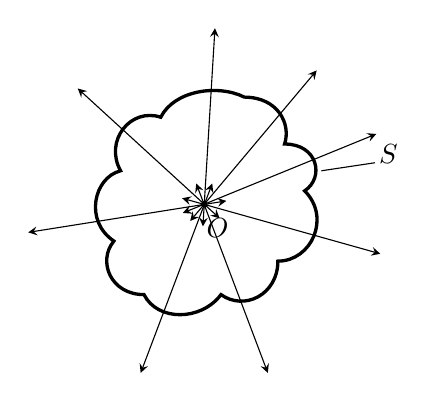
\begin{tikzpicture}[>=stealth,scale=0.85]
  \draw[<->] (-0.02,-0.33) -- (0.16,2.63);%
  \draw[<->] (-0.21,-0.25) -- (1.68,2.0);%
  \draw[<->] (-0.32,-0.13) -- (2.57,1.05);%
  \draw[<->] (-0.33,0.09) -- (2.63,-0.74);%
  \draw[<->] (-0.12,0.31) -- (0.95,-2.52);%
  \draw[<->] (0.12,0.31) -- (-0.95,-2.52);%
  \draw[<->] (0.33,0.05) -- (-2.63,-0.42);%
  \draw[<->] (0.23,-0.21) -- (-1.89,1.73);%
  \fill (0,0) circle (1.4pt);%
  \node at (0.2,-0.36) {$O$};
  \draw[very thick] (0.6,1.6) .. controls (1.1,1.6) and (1.3,1.2) .. (1.2,0.9)
        .. controls (1.7,0.9) and (1.8,0.4) .. (1.5,0.2)
        .. controls (1.9,-0.2) and (1.6,-0.85) .. (1.1,-0.85)
        .. controls (1.1,-1.35) and (0.6,-1.6) .. (0.25,-1.35)
        .. controls (-0.05,-1.75) and (-0.7,-1.75) .. (-0.9,-1.35)
        .. controls (-1.4,-1.35) and (-1.6,-0.85) .. (-1.35,-0.55)
        .. controls (-1.8,-0.25) and (-1.65,0.4) .. (-1.25,0.5)
        .. controls (-1.5,0.95) and (-1.1,1.45) .. (-0.65,1.3)
        .. controls (-0.45,1.7) and (0.2,1.8) .. (0.6,1.6);
  \node at (2.75,0.75) {$S$};
  \draw (2.55,0.62) -- (1.75,0.5);%
\end{tikzpicture}

图 4.7
\end{minipage}

当然都是\trContactType{}的。我们用一个例子来说明这一点：一张为%
$c_{0}$-\trLipschitz{}型但非\trContactType{}的\trHypersurface{} $S$。考察%
\trSymplectic\trCylinder{} $Z(R)\subset\bigl(\R^{2n},\omega_{0}\bigr)$ 的%
\trClosure{}之内一张\trDiffeomorphic{}于带凹坑球面的\trHypersurface，如下图所示

\noindent\begin{minipage}{\linewidth}
\centering
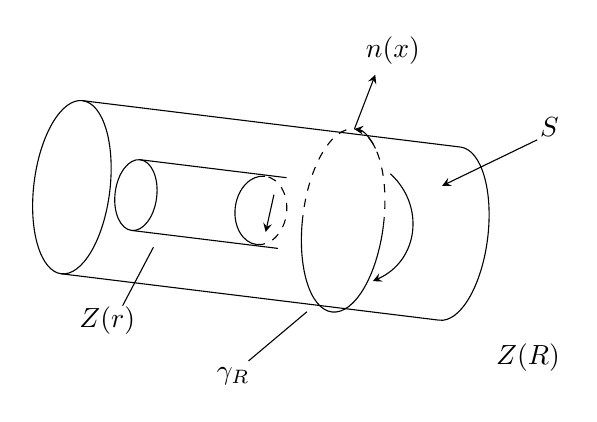
\begin{tikzpicture}[>=stealth,scale=0.78]
  \begin{scope}[rotate around={-7:(4.6,0)}]
    \draw (1.5,0) ellipse (0.62 and 1.42);
    \draw (1.5,1.42) -- (7.7,1.42);
    \draw (1.5,-1.42) -- (7.7,-1.42);
    \draw (7.7,1.42) arc[start angle=90,end angle=-90,x radius=0.62,y radius=1.42];
    \draw (2.55,0) ellipse (0.34 and 0.58);
    \draw (2.55,0.58) -- (4.95,0.58);
    \draw (2.55,-0.58) -- (4.95,-0.58);
    \draw[dashed] ([shift={(5.95,0)}]0:0.66 and 1.5)
          arc[start angle=0,end angle=180,x radius=0.66,y radius=1.5];
    \draw ([shift={(5.95,0)}]180:0.66 and 1.5)
          arc[start angle=180,end angle=360,x radius=0.66,y radius=1.5];
    \draw[->] ([shift={(5.95,0)}]55:0.66 and 1.5)
          arc[start angle=55,end angle=90,x radius=0.66,y radius=1.5];
    \draw[->] (5.95,1.5) -- (6.18,2.42);
    \draw[->] (6.62,0.85) .. controls (7.25,0.4) and (7.25,-0.5) .. (6.55,-0.92);
    \draw ([shift={(4.6,0)}]90:0.42 and 0.56)
          arc[start angle=90,end angle=270,x radius=0.42,y radius=0.56];
    \draw[dashed] ([shift={(4.6,0)}]270:0.42 and 0.56)
          arc[start angle=270,end angle=450,x radius=0.42,y radius=0.56];
    \draw[->] (4.78,0.28) -- (4.72,-0.34);
  \end{scope}
  \node at (6.75,2.6) {$n(x)$};
  \node at (9.3,1.35) {$S$};
  \draw[->] (9.1,1.15) -- (7.55,0.4);%
  \node at (2.1,-1.8) {$Z(r)$};
  \draw (2.35,-1.55) -- (2.85,-0.6);%
  \node at (4.15,-2.7) {$\gamma_{R}$};
  \draw (4.4,-2.45) -- (5.35,-1.65);%
  \node at (8.95,-2.4) {$Z(R)$};
\end{tikzpicture}

图 4.8
\end{minipage}

\[
Z(R)\ =\ \Bigl\{(x,y)\in\R^{2n}\ \Bigm|\ x_{1}^{2}+y_{1}^{2}<R^{2}\Bigr\}.
\]
以 $n(x)$ 记在 $x\in S$ 处的外法向，则 $Jn(x)\in T_{x}S$ 在 $S$ 上定义了一个%
属于\trCharacteristicLineBundle{}的\trSmooth\trVectorField，即%
$Jn(x)\in\mathcal{L}_{S}(x)$。现在用反证法，假设 $S$ 是\trContactType{}的。%
于是在 $S$ 附近存在一个 1-形式 $\alpha$，满足 $d\alpha=\omega_{0}$，而且要么
\[
\alpha\Bigl(Jn(x)\Bigr)\ >\ 0\ ,\qquad\text{对一切}\quad x\in S
\]
要么 $\alpha\bigl(Jn(x)\bigr)<0$ 对一切 $x\in S$ 成立。不失一般性，我们假设%
成立的是第一种情形。在 $\R^{2n}$ 上定义 1-形式 $\lambda$：
\[
\lambda\ =\ \sum_{j=1}^{n}y_{j}\,dx_{j}\ ,
\]
其中 $(x,y)\in\R^{2n}$。于是 $d\lambda=\omega_{0}$，从而在 $S$ 上%
$d\lambda=d\alpha$。于是，由 $H^{1}(S)=0$，我们可以找到一个\trSmooth{}函数%
$\rho:S\to\R$ 满足 $\alpha-\lambda=d\rho$。从而，对 $S$ 上\trVectorField{}%
$Jn$ 的每个\trPeriodicSolution{} $\gamma$，
\[
\int_{\gamma}\alpha\ =\ \int_{\gamma}\lambda\ >\ 0\ .
\]
然而，对上图中所描绘的、在外柱体与内柱体上的那两个特定的\trPeriodicSolution{}%
$\gamma_{R}$ 与 $\gamma_{r}$，我们有
\[
\int_{\gamma_{R}}\lambda\ =\ \pi R^{2}\qquad\text{以及}\qquad%
\int_{\gamma_{r}}\lambda\ =\ -\pi r^{2}\ .
\]
这一矛盾表明 $S$ 不是\trContactType{}的。显然，存在一个以 $S$ 为模型的%
\trParameterizedHypersurfaceFamily{} $(S_{\varepsilon})$，使%
$c_{0}\bigl(B_{\varepsilon},\omega_{0}\bigr)=\pi(R+\varepsilon)^{2}$ 与诸%
柱体的\trCapacity{}相一致，其中 $S_{\varepsilon}=\partial B_{\varepsilon}$。%
于是，$S=S_{0}$ 是 $c_{0}$-\trLipschitz{}型的。我们指出，上面的论证还表明：%
在一张\trContactType{}且满足 $H^{1}(S)=0$ 的\trCompact\trEnergySurface{} $S$%
上，诸\trPeriodicSolution{}的\trAction{}全都具有同一符号。特别地，在这样的%
\trHypersurface{}上诸\trAction{}决不为零。

我们以三维的一个晚近结果来结束本节，这个结果无法用迄今所描述的%
\trVariational{}方法得到。我们考察一个维数为 $2n-1$ 的\trSmooth{}\trClosed{}%
且\trOrientable{}的\trManifold{} $W$。$W$ 上的一个\textbf{\trContactForm}%
（contact form）是一个\trOneForm{} $\lambda$，它使 $\lambda\wedge(d\lambda)^{n-1}$%
成为 $W$ 上的一个\trVolumeForm。这样一个\trContactForm{}确定了一个所谓的%
\trContactStructure，即 $(2n-2)$ 维的\textbf{\trPlaneField}（plane field）%
$\xi_{\lambda}$，其定义为
\[
\xi_{\lambda}\ =\ \operatorname{Kern}(\lambda)\ \subset\ TW\ .
\]
此外，$d\lambda$ 的\trKernel{}是 $1$ 维的。于是存在唯一的\trVectorField{}%
$X=X_{\lambda}$ 满足
\[
i_{X}\,d\lambda\ \equiv\ 0\qquad\text{以及}\qquad i_{X}\lambda\ =\ 1\ .
\]
$W$ 上这个特定的处处非零的\trVectorField{}称为与 $\lambda$ 相联系的%
\trReeb\trVectorField。注意，我们不再要求 $W=\partial M$ 与%
$d\lambda=\omega|_{W}$\footnote{原书印作「$\omega|M$」，而 $d\lambda$ 定义在 $W$ 上，其限制对象应为 $\omega|_{W}$，此处径改。——译者注}，其中 $(M,\omega)$ 是一个维数为 $2n$ 的\trCompact%
\trSymplecticManifold。

我们将说，\trWeinstein{}猜想对\trManifold{} $W$ 成立，如果对 $W$ 上的每个%
\trContactForm{} $\lambda$，与之相联系的\trReeb\trVectorField{} $X_{\lambda}$%
都有一条\trClosed\trOrbit。

\begin{theorem}[H.~\trHofer]\label{thm:hofer-sphere-three}
\trWeinstein{}猜想对三维球面 $S^{3}$ 成立。
\end{theorem}

实际上，对每个满足 $\pi_{2}\bigl(W^{3}\bigr)\neq0$ 的\trClosed{}\trOrientable{}%
三维\trManifold{} $W^{3}$，\trWeinstein{}猜想也成立，参看 H.~\trHofer{}%
[118]（1993）。该证明基于「\trCauchyRiemann」型的一阶\trElliptic%
\trPartialDifferentialEquation，并受到\trGromov{}的\trSymplecticManifold{}中%
\trPseudoholomorphic\trCurve{}理论 [107] 与\trEliashberg{}关于利用%
\trHolomorphic\trDisc{}的填充技巧的概要 [73] 的影响。

我们指出，$S^{3}$ 上存在许多\trContactForm{} $\lambda$——即所谓的%
\textbf{\trOvertwisted}（overtwisted）\trContactForm——它们不容许 $S^{3}$ 到 $\R^{4}$%
中的一个嵌入，使得被诱导的\trHamiltonian\trFlow{}与由 $X_{\lambda}$ 所定义的%
\trReeb{}流共轭。

这里，一个\trClosed{}三维\trManifold{} $W$ 上的\trContactForm{} $\lambda$ 被%
\trEliashberg{}称为\trOvertwisted{}的，如果存在一个嵌入的\trDisc{} $F\simeq D^{2}$，其中%
$D^{2}=\bigl\{z\in\C\ \bigm|\ \lvert z\rvert\leq1\bigr\}$，使得
\begin{align*}
T(\partial F)\ &\ \subset\ \xi_{\lambda}\big|\partial F\\
T_{x}F\ &\ \nsubseteq\ \xi_{\lambda,x}\qquad\text{对一切}\quad x\in\partial F\ .
\end{align*}
在\trLutz{}[144] 与\trMartinet{}[147] 的经典工作中，每个\trCompact%
\trOrientable{}的三维\trManifold{}上都建立了\trContactStructure。特别地，%
$S^{3}$ 上存在彼此不经\trDiffeomorphism{}（其意义见下文所述）等价的\trOvertwisted%
\trContactStructure。

一个不\trOvertwisted{}的\trContactForm{} $\lambda$ 称为\textbf{\trTight}（tight）的。据%
\trEliashberg{} [74] 的一个深刻的分类结果，在相差\trDiffeomorphism{}的意义下，%
$S^{3}$ 上却只有一个紧的\trContactStructure。更确切地说，若 $\lambda_{1}$，%
$\lambda_{2}$ 是 $S^{3}$ 上的紧形式，则按\trEliashberg，存在一个\trSmooth{}%
函数 $f:S^{3}\to\R\backslash\bigl\{0\bigr\}$ 与一个\trDiffeomorphism{}%
$\psi:S^{3}\to S^{3}$ 满足
\[
\psi^{*}\lambda_{2}\ =\ f\,\lambda_{1}\ .
\]
现在我们将证明：对于 $S^{3}$ 上的一个紧\trContactStructure，与之相联系的%
\trReeb\trVectorField{}具有一个\trPeriodicSolution。把 $S^{3}$ 表示为 $\C^{2}$%
的子集 $\bigl\{(z_{1},z_{2})\ \bigm|\ |z_{1}|^{2}+|z_{2}|^{2}=1\bigr\}$。记%
$z_{j}=q_{j}+ip_{j}$，其中 $q_{j}$, $p_{j}\in\R$，我们在 $\C^{2}$ 上定义%
1-形式
\[
\lambda_{0}\ =\ \frac{1}{2}\sum_{j=1}^{2}\bigl(p_{j}\,dq_{j}-q_{j}\,dp_{j}\bigr)
\]
使得 $d\lambda_{0}=\omega_{0}$。由于\trBennequin{}[20] 的一个基本结果，%
特殊的\trContactForm{} $\lambda_{0}|S^{3}$ 是紧的。于是，给定 $S^{3}$ 上任一%
紧\trContactForm{} $\lambda$，我们便找到一个无处为零的函数%
$f:S^{3}\to\R\backslash\bigl\{0\bigr\}$ 与一个 $S^{3}$ 的\trDiffeomorphism{}%
$\psi$，使得
\[
\psi^{*}\lambda\ =\ f\cdot\bigl(\lambda_{0}|S^{3}\bigr)\ .
\]
于是，$\lambda$ 与 $f\cdot\bigl(\lambda_{0}|S^{3}\bigr)$ 的\trReeb{}流相互%
共轭。我们可以利用这一点来证明：在这一特殊情形，$X_{\lambda}$ 具有一条%
\trPeriodicOrbit。由于 $X_{f\lambda_{0}}=-X_{-f\lambda_{0}}$，我们可以假设%
$f$ 取正值。我们断言：存在一张\trSmooth\trHypersurface{} $S\subset\C^{2}$，%
它是一个\trStarShaped{}的\trDomain{}的\trBoundary，并且存在一个%
\trDiffeomorphism{} $\psi:S^{3}\to S$，使得
\[
T\psi\Bigl(\mathcal{L}_{f\lambda_{0}}\Bigr)\ =\ \mathcal{L}_{S}\ ,
\]
其中 $\mathcal{L}_{f\lambda_{0}}$ 是 $S^{3}$ 的由与 $f\lambda_{0}$ 相联系的%
\trReeb\trVectorField{}所定义的\trLineBundle，而 $\mathcal{L}_{S}$ 是由%
$\C^{2}\cong\R^{4}$ 中的\trStandard\trSymplecticStructure{} $\omega_{0}$ 在%
\trHypersurface{} $S$ 上诱导出的\trCharacteristicLineBundle。的确，我们只需%
把\trHypersurface{} $S$ 定义为
\[
S\ =\ \Bigl\{\sqrt{f(z)}\,z\ \Bigm|\ z\in S^{3}\Bigr\}\ \subset\ \C^{2}
\]
并把\trDiffeomorphism{} $\psi:S^{3}\to S$ 定义为%
$\psi(z)=\sqrt{f(z)}\,z$。现在注意到 $\lambda_{0}(z)=\tfrac{1}{2}%
\omega_{0}(z,\cdot)$（$z\in\C^{2}$），我们简记 $\sigma=\sqrt{f}$，并对%
$z\in S^{3}$、$h\in T_{z}S^{3}$ 计算
\begin{align*}
\psi^{*}\bigl(\lambda_{0}|S\bigr)(z;h)\ &=\ \tfrac{1}{2}\omega_{0}\Bigl(\sigma(z)z,\ \bigl(d\sigma(z)h\bigr)z+\sigma(z)h\Bigr)\\
&=\ \sigma(z)^{2}\,\tfrac{1}{2}\omega_{0}(z,h)\\
&=\ \bigl(f\cdot\lambda_{0}\bigr)(z,h)\ .
\end{align*}
由此，上述断言得证。利用上文证明的 P.~\trRabinowitz{}的存在性结果，我们得出%
结论：\trReeb\trVectorField{} $X_{f\lambda_{0}}$ 具有一个\trPeriodicSolution。

总而言之，我们已证明：在 $S^{3}$ 上的\trContactStructure{} $\lambda$ 为紧的%
这一例外情形，与之相联系的\trReeb\trVectorField{} $X_{\lambda}$ 至少拥有一条%
\trClosed\trOrbit。
